\documentclass{beamer}
\usepackage{ulem}
\usepackage{tikz}
\usepackage{caption}
\usepackage{subcaption}
\usepackage{multicol}
\usepackage{hyperref}
\usetikzlibrary{positioning}
\usetheme{Dresden}
\usecolortheme{wolverine}
\title{sMDT Chamber Production at the University of Michigan}
\author{Evan Carpenter}
\date{February 7th, 2023}

\graphicspath{{./images}}

\definecolor{googlegreen}{rgb}{0.7137,0.8431,0.6588}
\definecolor{googleblue}{rgb}{0.4275,0.6196,0.9216}
\definecolor{googleyellow}{rgb}{1,1,0}
\definecolor{googlered}{rgb}{0.8784,0.4,0.4}
\setbeamertemplate{navigation symbols}{}
\addtobeamertemplate{navigation symbols}{}{%
    \usebeamerfont{footline}%
    \usebeamercolor[fg]{footline}%
    \hspace{1em}%
    \insertframenumber/\inserttotalframenumber
}

\def\ph{\textcolor{red}{PLACEHOLDER}}


\titlegraphic{
	\begin{tikzpicture}[remember picture, overlay]
		\node[xshift=-0.4\pdfpagewidth, yshift=-0.031\pdfpageheight]{
\includegraphics[width=0.17\linewidth]{atlas.png}};
		\node [xshift=0.35\pdfpagewidth, yshift=-0.05\pdfpageheight]{
\includegraphics[width=0.2\linewidth]{UM.png}};
	\end{tikzpicture}
}

\newcommand{\backupbegin}{
   \newcounter{finalframe}
   \setcounter{finalframe}{\value{framenumber}}
}
\newcommand{\backupend}{
   \setcounter{framenumber}{\value{finalframe}}
}
\newcommand{\hyperlinktarget}[3]{\hyperlink{#1}{\hypertarget{#2}{#3}}}




\begin{document}
%\begin{frame}
	\titlepage
\end{frame}
\begin{frame}
	\tableofcontents
\end{frame}
\section*{Background and Overview}
	\begin{frame}{Chamber and Tube Construction}
		\begin{itemize}
			\item Goal is to produce 50 total chambers.\footnote{\tiny 8 BIS1 + 1 extra, 40 (BIS2-6) + 1 extra}
			\item Last Muon week talk covered chambers 0-30
			\item Since then, chambers up to 35 have been fully made.
			\item Began construction of additional tubes in November to supplement chamber production.
			\item 2 papers accepted for publication on methods. 
		\end{itemize}
		\begin{figure}
			\centering
			\begin{subfigure}[c]{0.4\pdfpagewidth}
				
\includegraphics[width=0.4\pdfpagewidth]{ChamberPaperTitlePage.png}
				\caption*{Chamber Paper: \href{https://arxiv.org/abs/2211.00714}{arXiv:2211.00714}}
			\end{subfigure}
			%\hfill
			\begin{subfigure}[c]{0.4\pdfpagewidth}
				
\includegraphics[width=0.4\pdfpagewidth]{TubePaperTitlePage.png}
				\caption*{Tube Paper: \href{https://arxiv.org/abs/2209.03864}{arXiv:2209.03864}}
			\end{subfigure}
		\end{figure}
	\end{frame}%
%\section{UM Tube Production}
	\subsection{Construction Process}
		\begin{frame}{Overview}
			\begin{itemize}
				\item In order to supplement supply being recieved from Michigan State University, UM started it's second wave of tube construction in November 2022.
				\item 4-5 full time workers for construction and testing, 3 part time students for additional testing. 
				\item Goal of 1000 sMDTs constructed before 2023. Average 50 Tubes/Day. 
			\end{itemize}
		\end{frame}
		\begin{frame}{Construction and Testing}
			\begin{figure}
				\centering
				\begin{subfigure}[c]{0.4\pdfpagewidth}
					\centering
					\includegraphics[width=0.5\pdfpagewidth]{TubeProduction.png}
				\end{subfigure}
				~
				\begin{subfigure}[c]{0.4\pdfpagewidth}
					\centering
					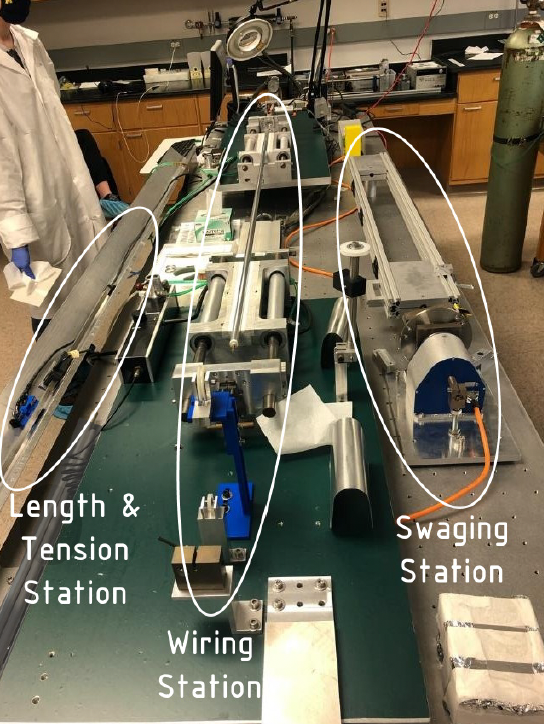
\includegraphics[height=0.4\pdfpageheight]{TubeProductionAlternateView.png}
				\end{subfigure}
			\end{figure}
		\end{frame}
		\begin{frame}{sMDT QA/QC Tests}
			\begin{figure}
				\begin{subfigure}[c]{0.4\pdfpagewidth}
					\centering
					\hyperlinktarget{DCExtra}{DC}{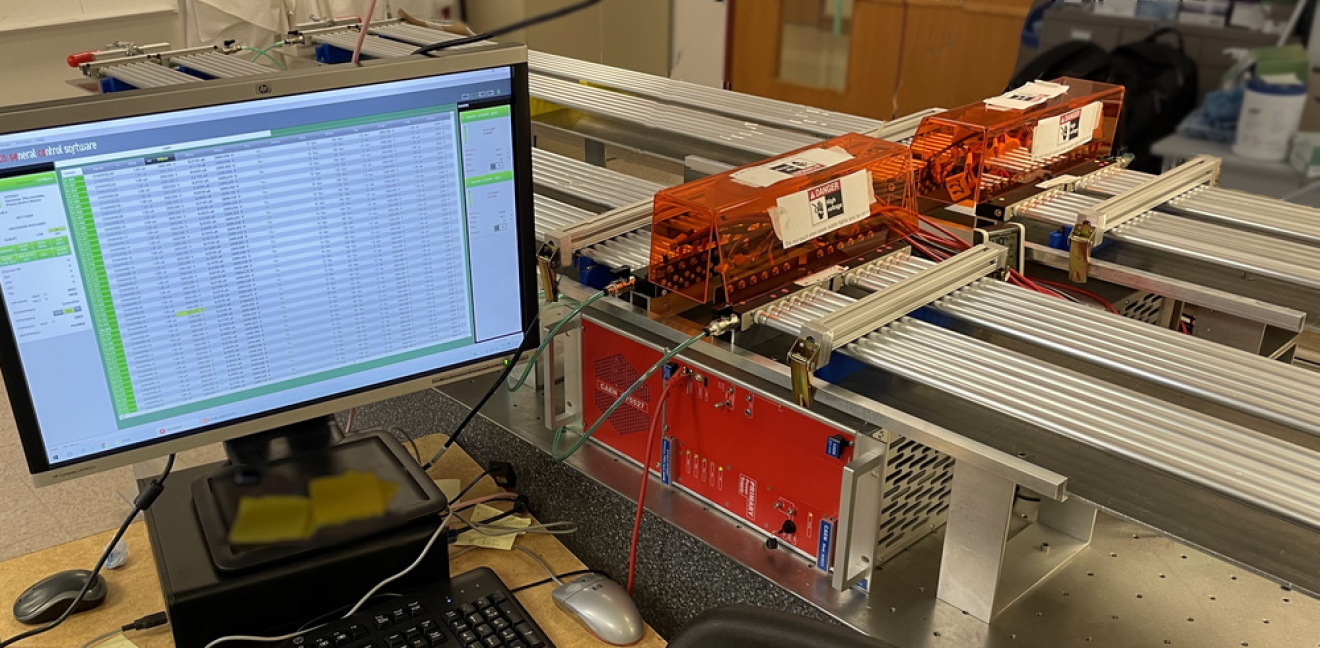
\includegraphics[width=0.7\textwidth]{CAENForDC.png}}
					\caption{Dark Current Testing setup.}
				\end{subfigure}
				\begin{subfigure}[c]{0.4\pdfpagewidth}
					\centering
					\hyperlinktarget{LeakRateTubesExtra}{LeakRateTubes}{\includegraphics[width=0.5\textwidth]{LeakDetector.png}}
					\caption{Helium Leak Testing Setup}
				\end{subfigure}
			\end{figure}

			\begin{figure}
				\centering
				\hyperlinktarget{TensionExtra}{TensionPhoto}{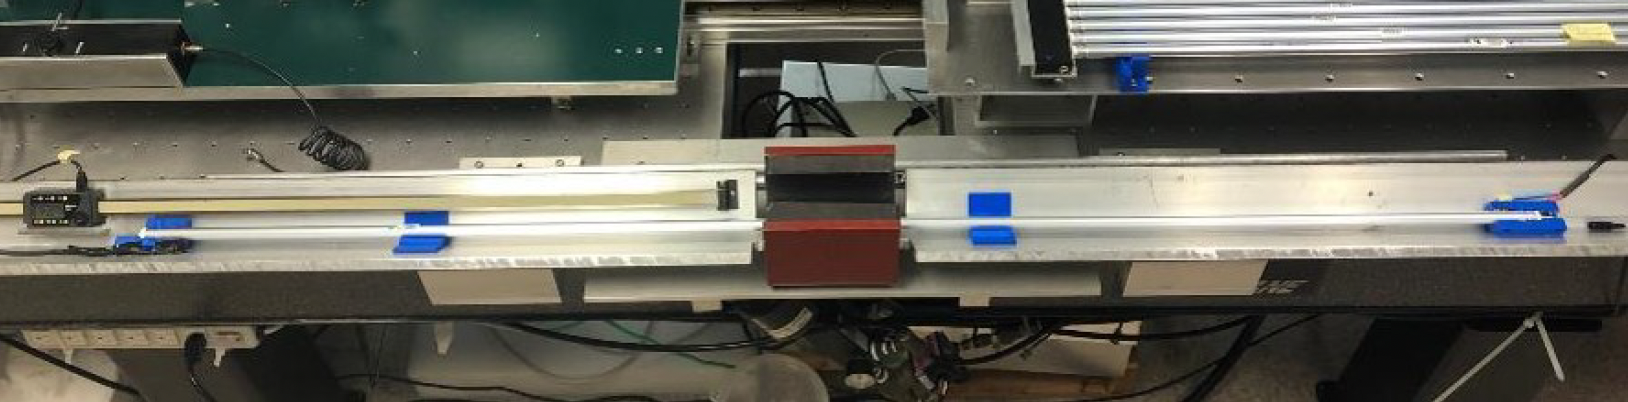
\includegraphics[width=0.6\textwidth]{TensionStation.png}}
				\caption{Tension Testing Setup}
			\end{figure}
		\end{frame}
		\begin{frame}{Results}
			\begin{itemize}
				\item Completed after 32 working days in December 2022 with 1,359 tubes total. 
				\item Constructed sMDTs still undergoing QA/QC. 
				\item 19 total failed QA tests. (Failure Rate of 1.8\%)
			\end{itemize}
		\end{frame}




\section{Chamber Production}
	
	\subsection{Construction Process}
		\begin{frame}{High Bay}
			
		\end{frame}
		\begin{frame}
			\scalebox{0.65}{
				\begin{minipage}{0.5\pdfpagewidth}
							\begin{description}
							\item [Week 1:] \colorbox{googlegreen}{Tube Gluing}
								\begin{itemize}\small
									\item Glue 2 layers per day (including gluing spacer frame/RASNIK layer)
								\end{itemize}
							\item [Week 2:] \colorbox{googlegreen}{Position Measurements}
								\begin{itemize}\small
									\item Measure wire heights 
									\item Glue AP-plates, B-field sensors, CCC platforms.
									\item Measure platforms.
									\item Glue support bars.
								\end{itemize}
							\item [Week 3:] \colorbox{googleblue}{Gas Systems}
							\item [Week 4:] \colorbox{googleyellow}{Cosmic Ray Test}
						\end{description}
					\end{minipage}
					}
			\hfill
			\begin{minipage}{0.4\pdfpagewidth}
				\begin{figure}
					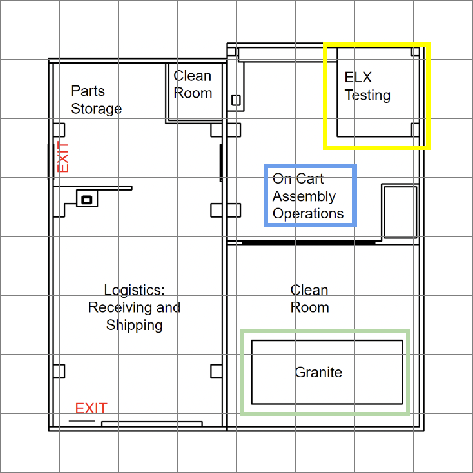
\includegraphics[width=0.4\pdfpagewidth]{test.pdf}
				\end{figure}
			\end{minipage}
		\end{frame}
		\begin{frame}{\ph}
			\begin{figure}[t]
				\centering
				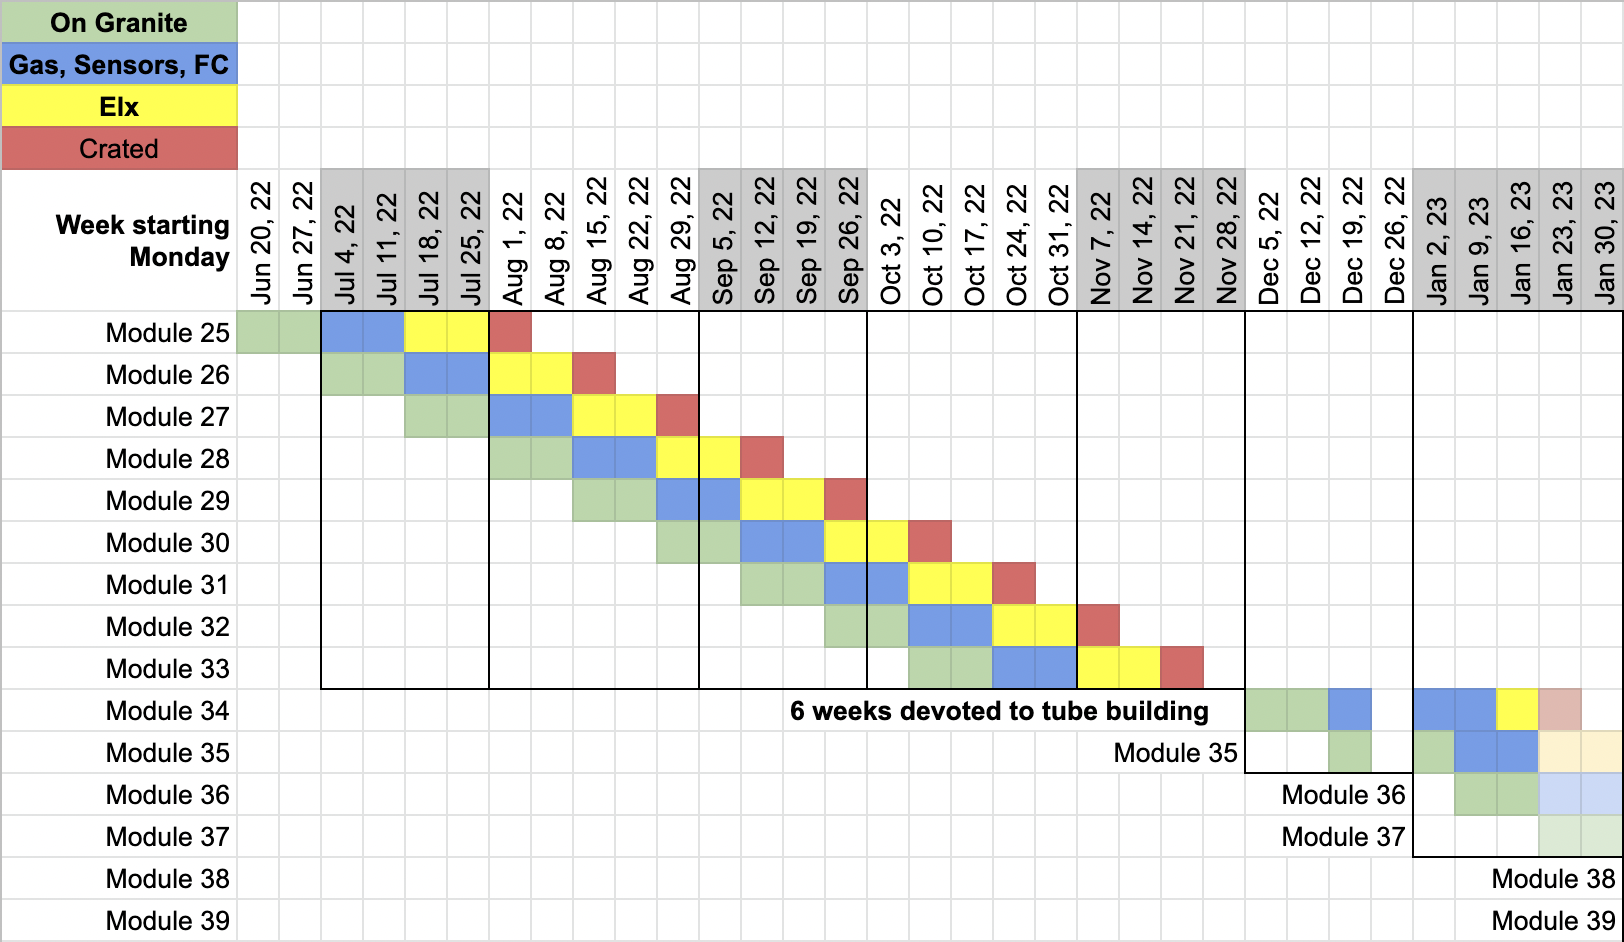
\includegraphics[width=0.8\pdfpagewidth]{Chamber Production.png}		
				\label{fig:ChamberProduction}		
			\end{figure}
		\end{frame}
	\subsection{Testing}

		\begin{frame}{Measurements \ph}
			\begin{itemize}
				\item Platform positioning
				\item Endplug height positioning (different from mpi)
				\item we domt have coordinate measuee machine, measure endplug height, assume z direction is fine, set by combs
				\item layer spacing layer pitch
				\item Leak Rate
				\item Effeciency
				\item Resolution
			\end{itemize}
		\end{frame}
		\begin{frame}{Wire Height \ph}
			\begin{figure}
				\centering
				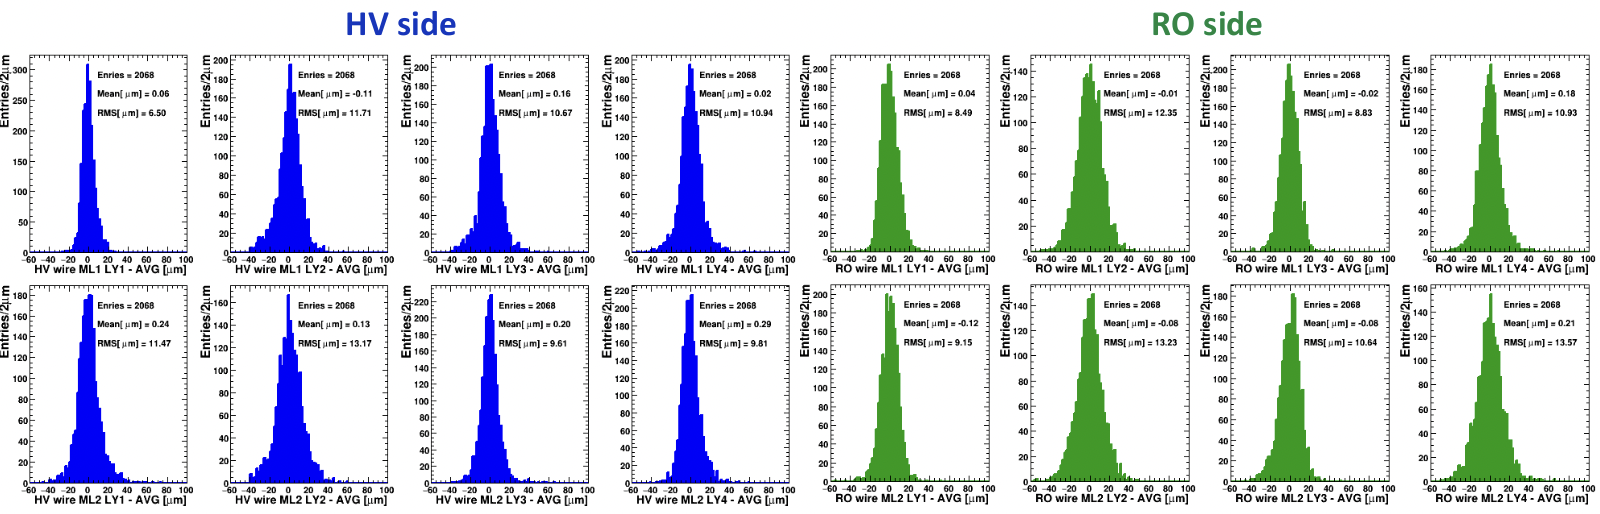
\includegraphics[width=0.6\pdfpagewidth]{WireHeightOffset.png}
			\end{figure}
		\end{frame}
		\begin{frame}{Inplane Alignment \ph}
			\framebox{\begin{figure}
				\begin{subfigure}[c]{0.3\pdfpagewidth}
					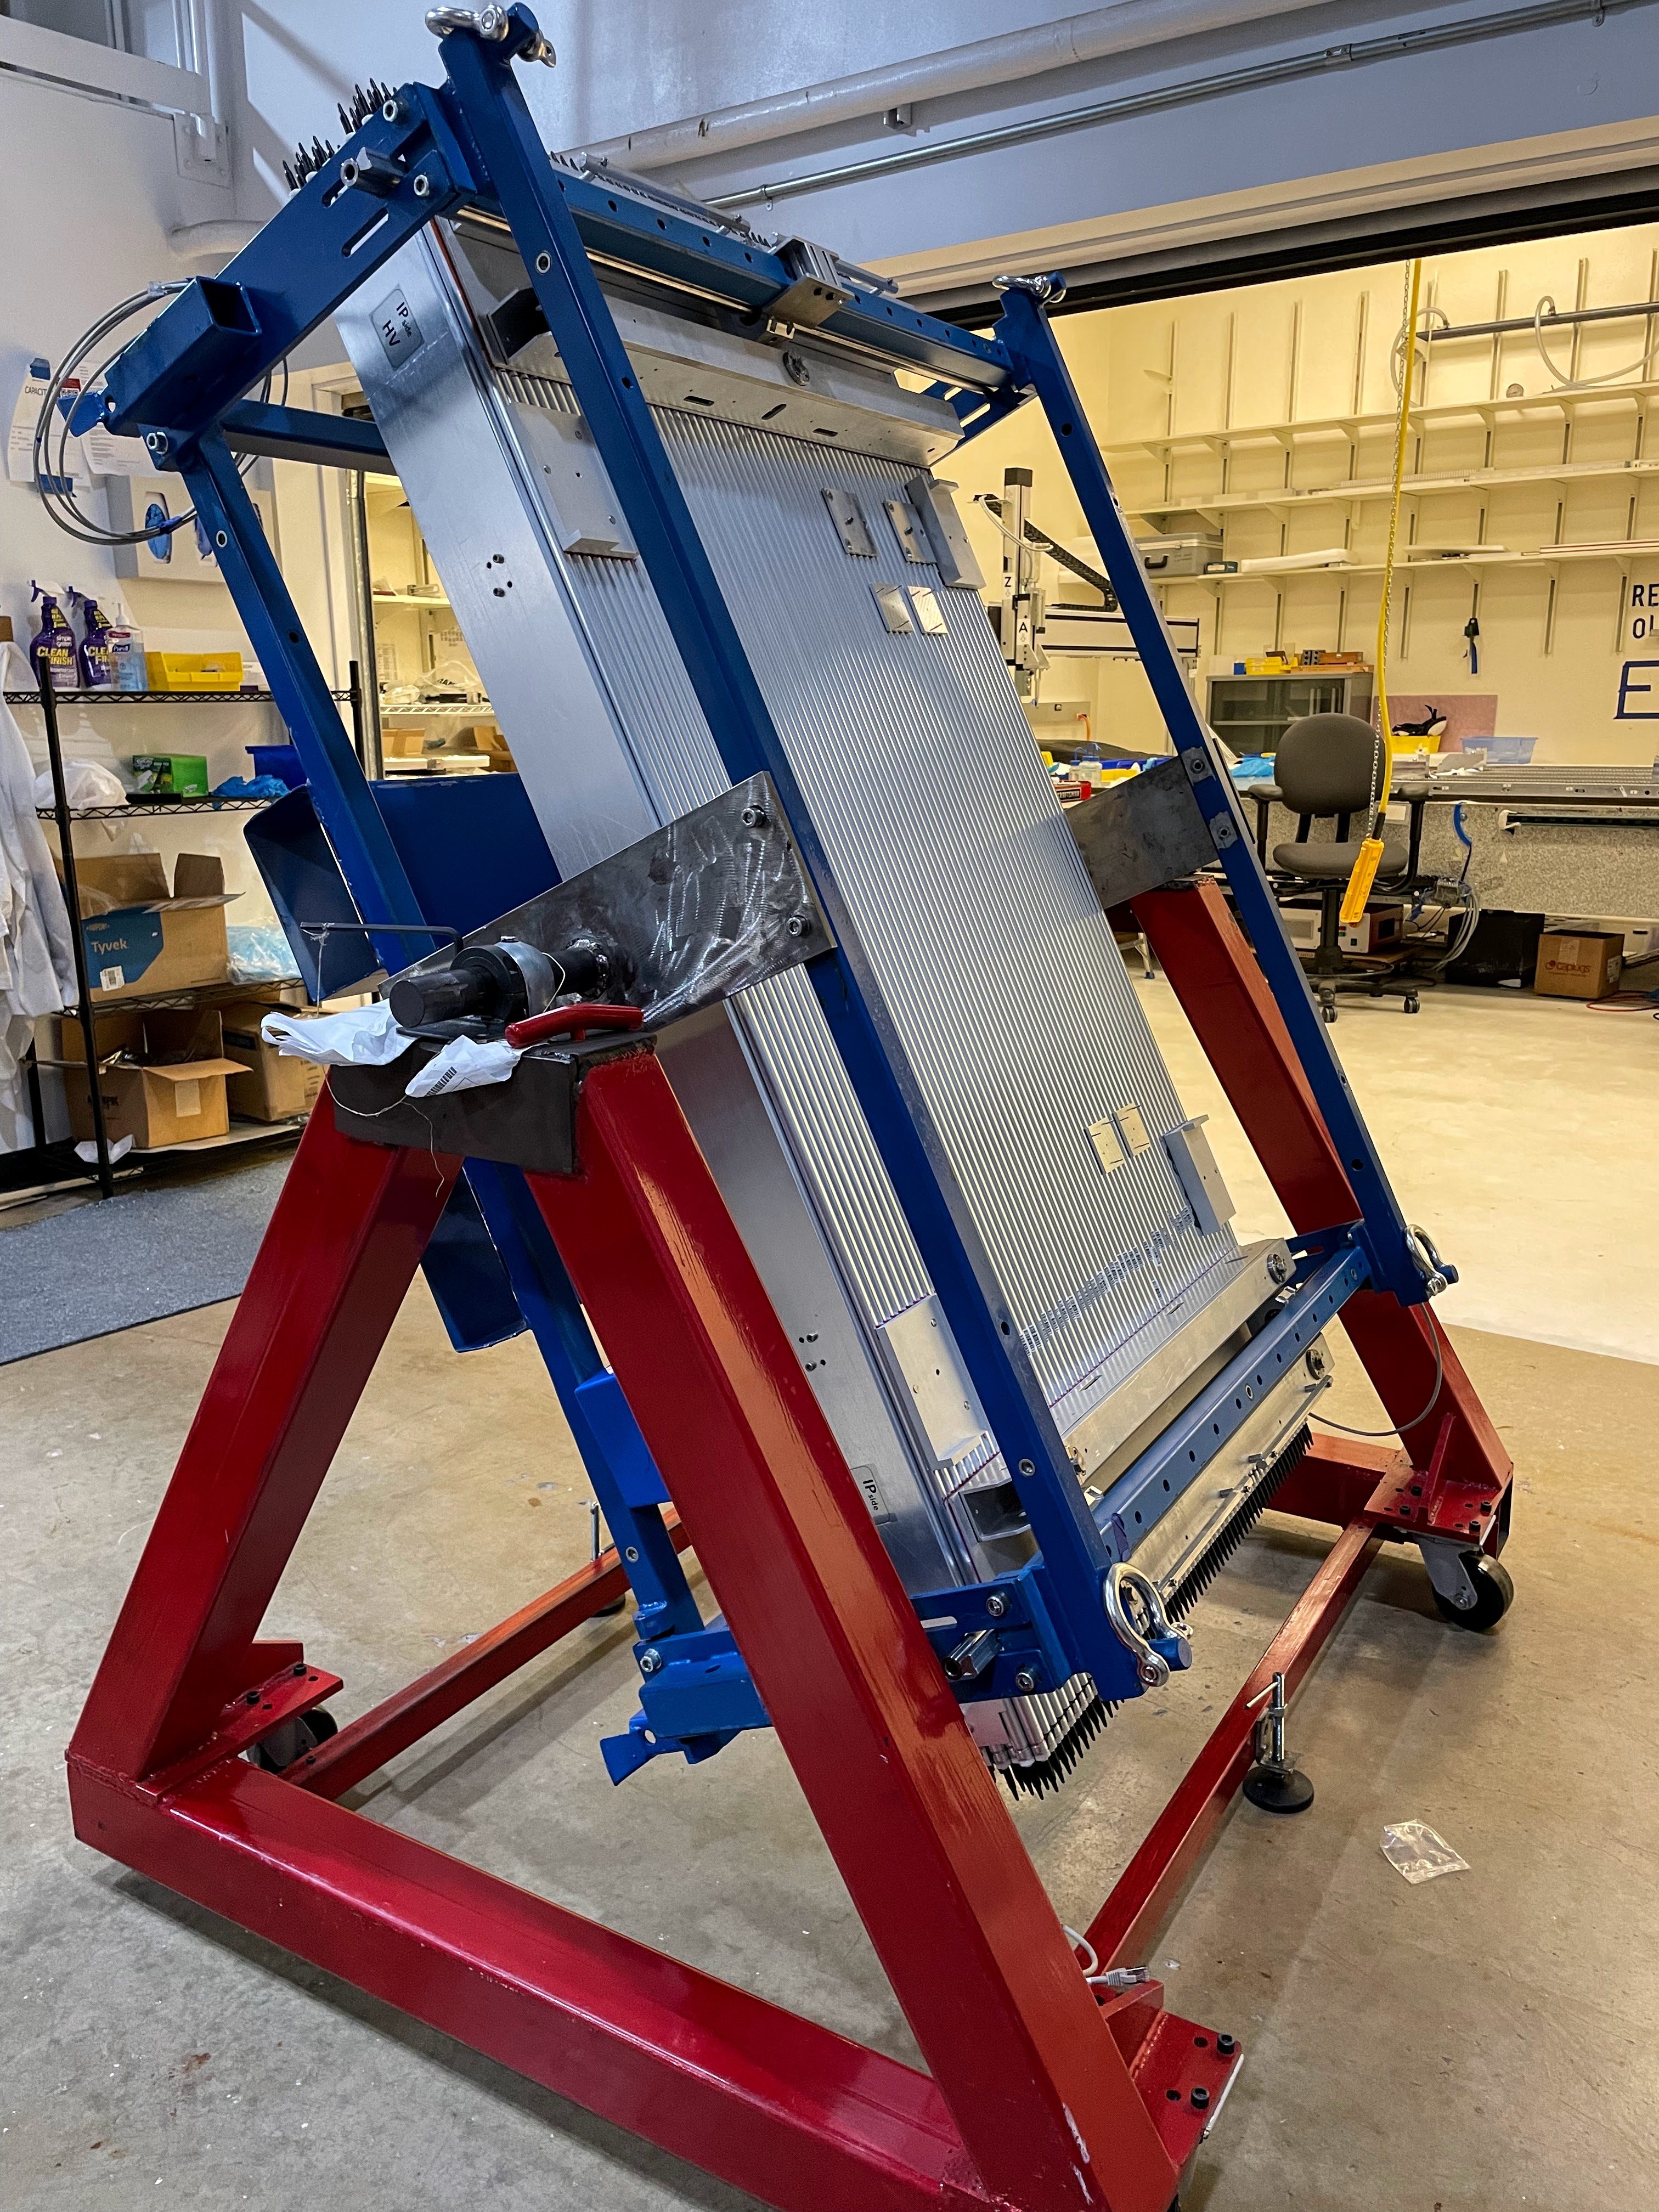
\includegraphics[height=0.4\pdfpageheight]{RotationCart.jpg}
					\caption{Chamber on rotation cart}
					\label{fig:RotationCart}
				\end{subfigure}
				~
				\begin{subfigure}[c]{0.5\pdfpagewidth}
					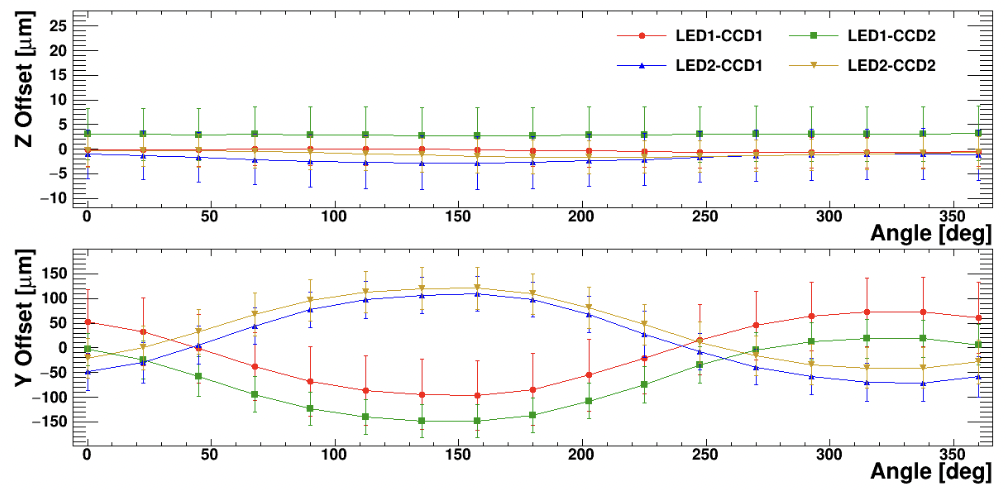
\includegraphics[width=0.4\pdfpagewidth]{RASNIKMeasurements.png}
					\caption{Deviation}
					\label{fig:InplaneAlignment}
				\end{subfigure}
			\end{figure}}
		\end{frame}

		\begin{frame}{Leak Rate \ph}
			\begin{figure}
				\centering	
				\begin{subfigure}[t]{0.4\pdfpagewidth}
					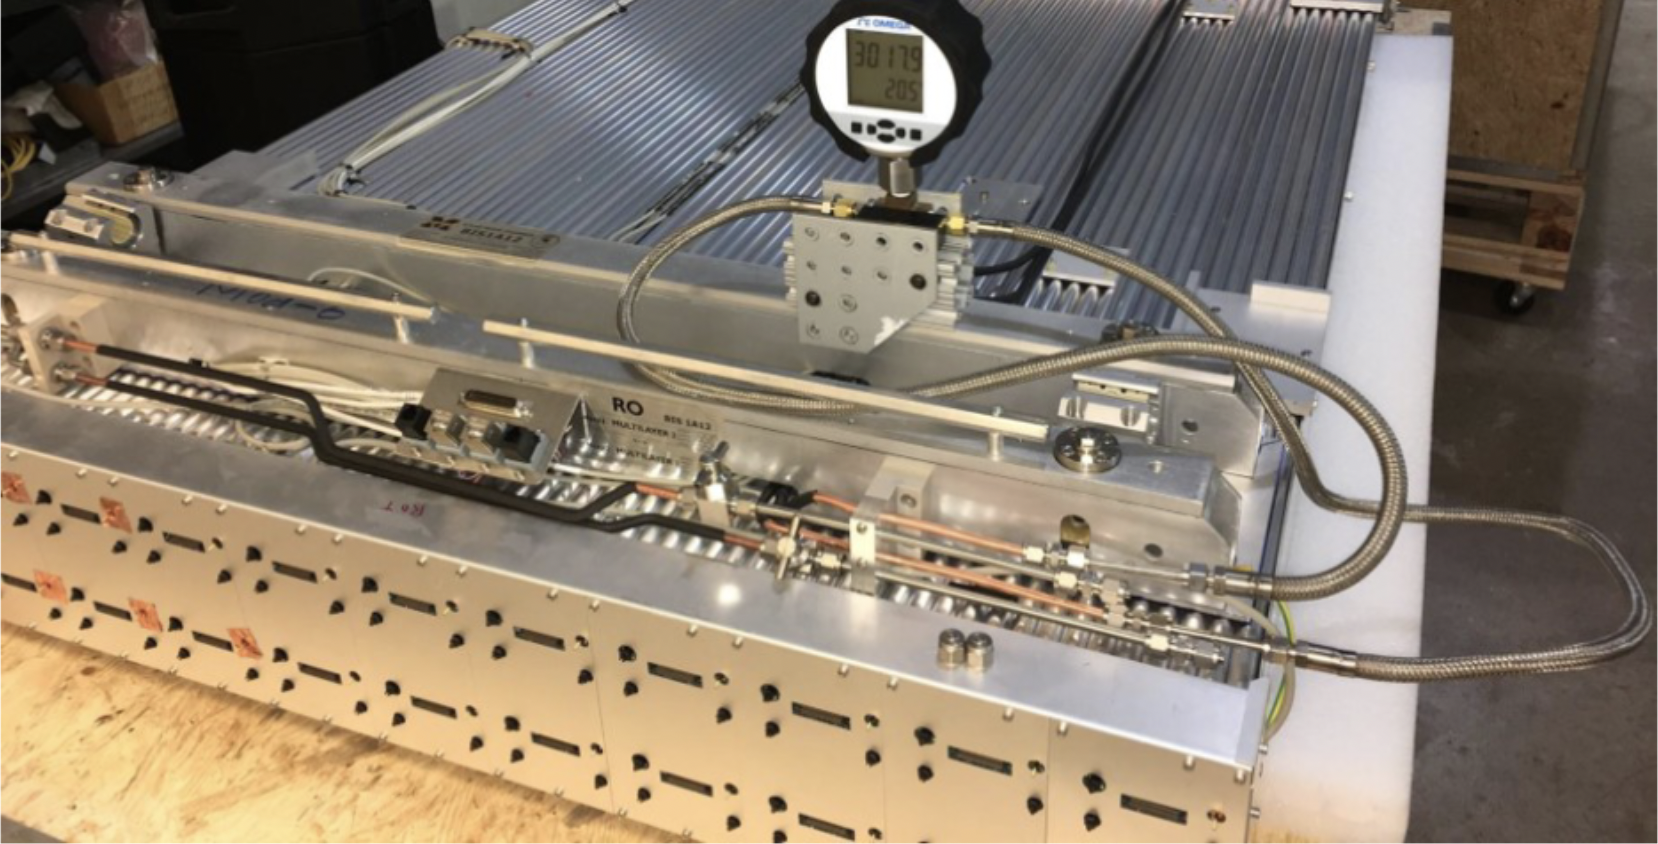
\includegraphics[width=0.4\pdfpagewidth]{PressureGauge.png}
					\caption{Chamber undergoing a pressure drop leak test}
				\end{subfigure}
				\hfill
				\begin{subfigure}[t]{0.4\pdfpagewidth}
					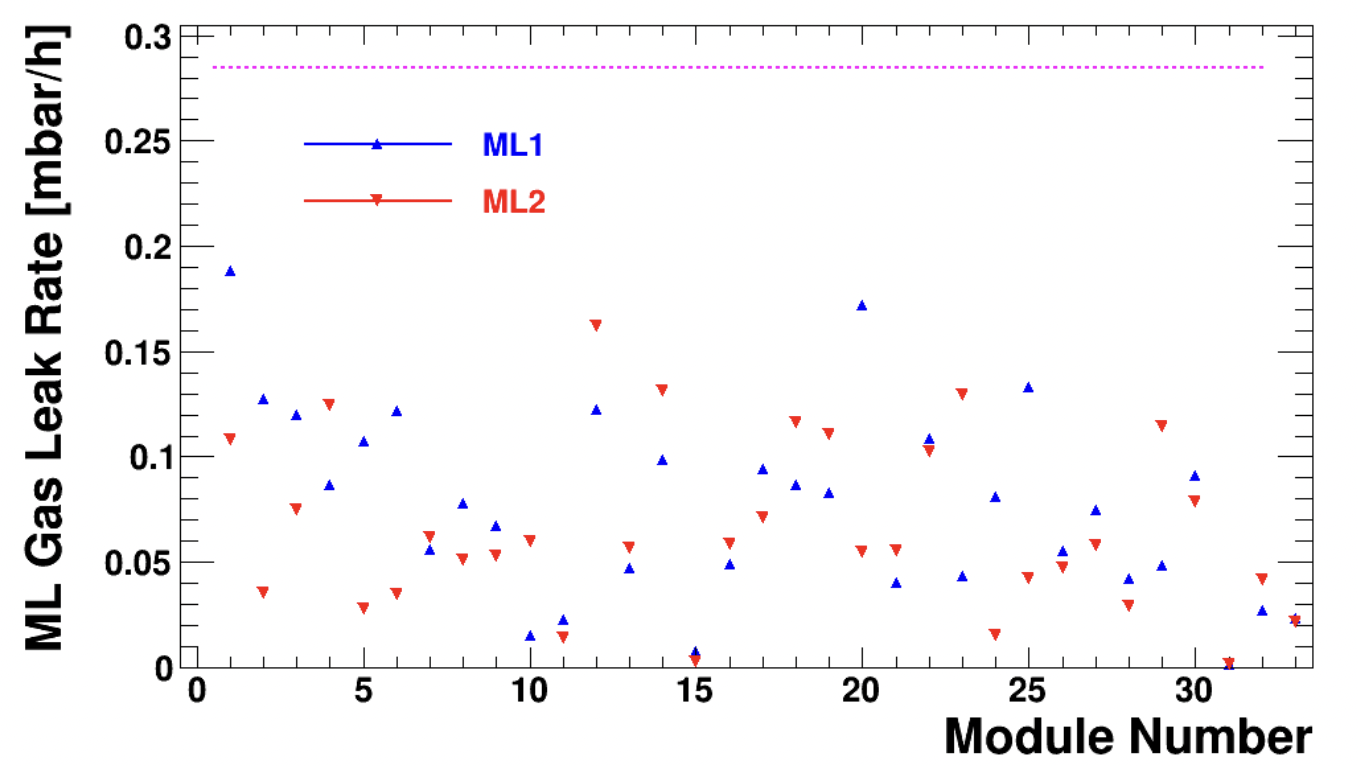
\includegraphics[width=0.4\pdfpagewidth]{ChamberLeakRate.png}
					\caption{Leak Rates of past 35 modules. The dotted pink line is the maximum acceptable leak rate of 0.288 mbar/hr.}
				\end{subfigure}
			\end{figure}
		\end{frame}

		\begin{frame}{Efficiency \ph}
			\begin{figure}[t]
				\centering	
				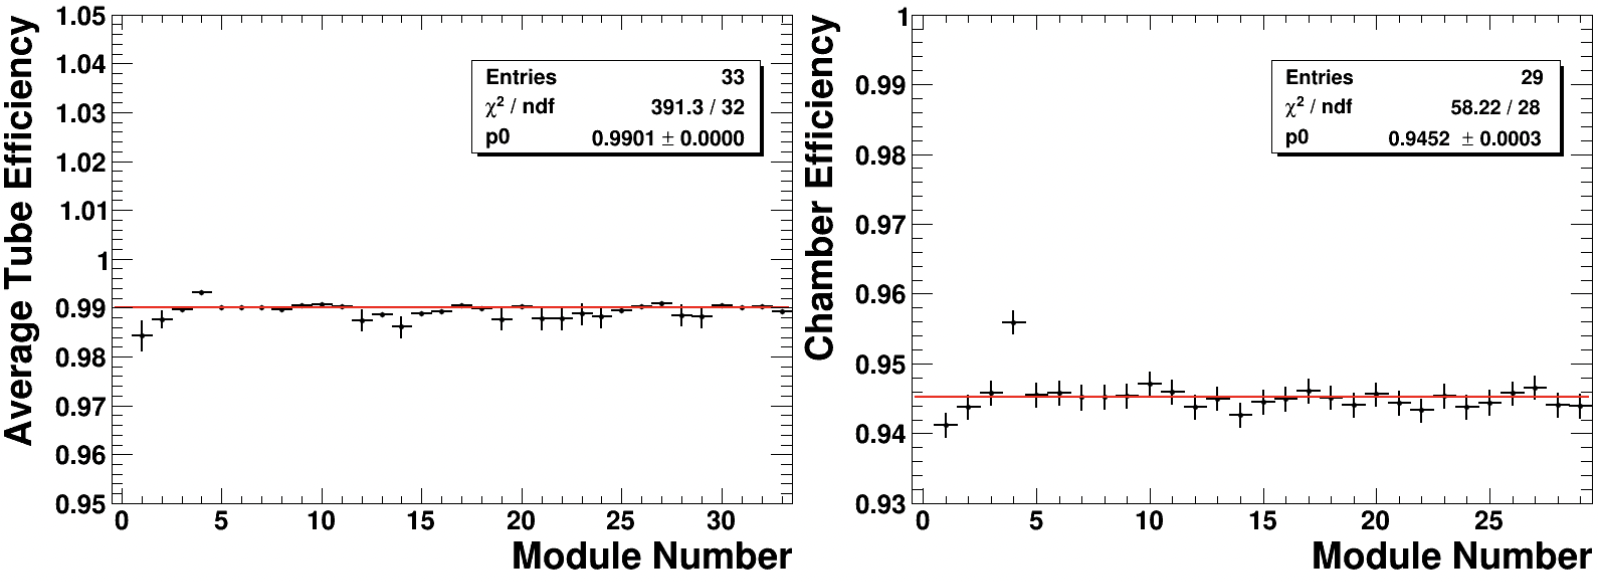
\includegraphics[width=0.8\pdfpagewidth]{ChamberEfficiency.png}
				\label{fig:ChamberEfficiency}
			\end{figure}
		\end{frame}
		
		\begin{frame}{Resolution \ph}
			\begin{figure}
				\centering	
				\begin{subfigure}[c]{0.4\pdfpagewidth}
					\centering
					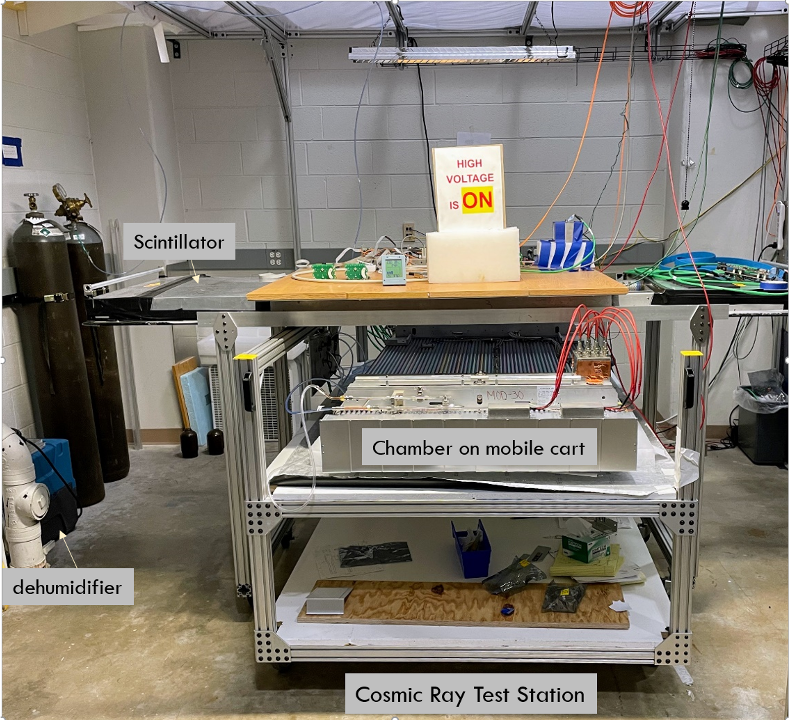
\includegraphics[width=0.3\pdfpagewidth]{CosmicRay-Station.png}
					\caption{Cosmic Ray testing station}
				\end{subfigure}
				\hfill
				\begin{subfigure}[c]{0.4\pdfpagewidth}
					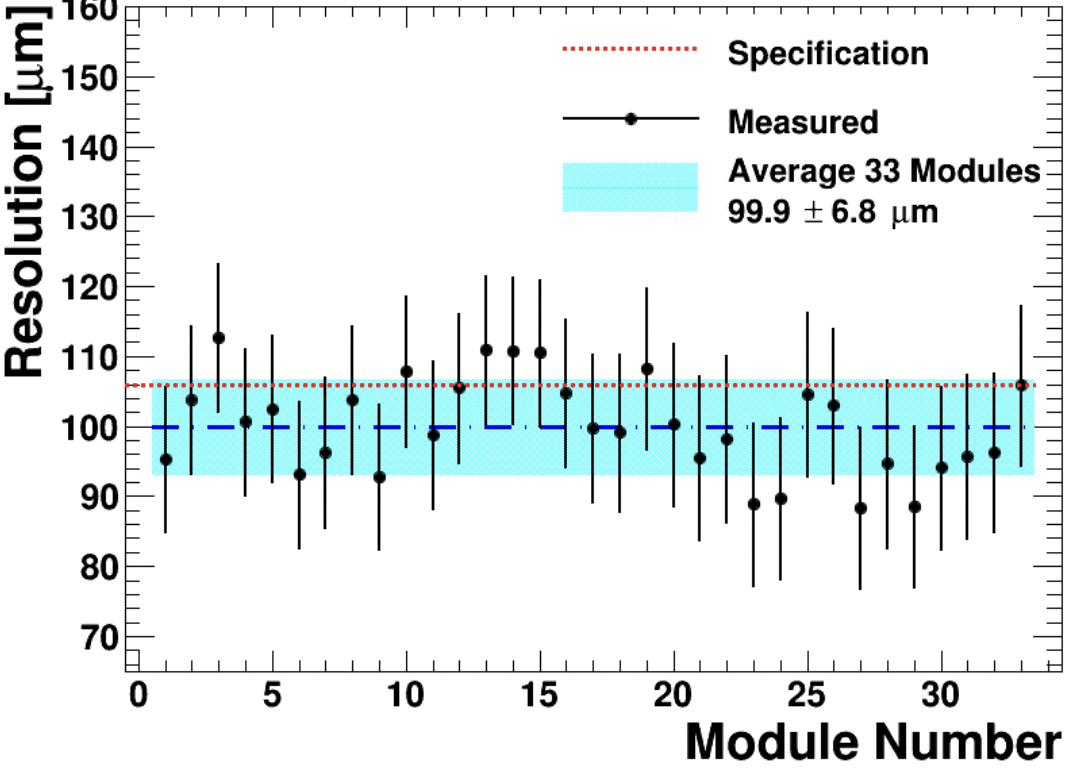
\includegraphics[width=0.4\pdfpagewidth]{ChamberResolution.png}
					\caption{Resolution done with convolutions}
					\label{fig:ChamberResolution}
				\end{subfigure}
			\end{figure}
			mpi takes shorter run, we take out scattering with convolutions
		\end{frame}



	\subsection{Moving Forward}

		\begin{frame}{New Electronics}
			replacing csms (csm catches stuff from mezzanine and sends as light)
			so we neeed new mezzanine cards 
		\end{frame}





%\section{Inventory}
	\begin{frame}
		\begin{figure}
			\begin{subfigure}[t]{0.25\pdfpagewidth}
				\centering
				\scalebox{0.5}{
				\begin{tabular}{l|r|r}
					\toprule
					GAS SYSTEM	&	On Hand	&	Excess\\
					\midrule
					Signal caps	&	15,769	&	2,777\\
					Grounding Pins	& 9,841	&97\\
					Grounding screw anchors	&	10,460	&	1,412\\
					58-hole distribution bars	&	56	&	0\\
					Plastic Gas Fitting Sets	& & 	\\
					Gas Tubing and Fittings	&	25	&	11\\
					Gas Mounting Blocks	& 15	&	1\\
					Gas Valves	&	56	&	0\\
					\bottomrule
				\end{tabular}}
			\end{subfigure}
			\qquad\qquad
			\begin{subfigure}[t]{0.25\pdfpagewidth}
				\centering
				\scalebox{0.5}{
					\begin{tabular}{l|r|r}
						\toprule
						SPACER FRAME&	On Hand	&	Excess\\
						\midrule		
						BIS2 spacer frame bar Cam	& 13	&0\\
						BIS2 spacer frame bar LED	& 13	&0\\
						BIS2 spacer frame bar Central Lens	& 13	&0\\
						BIS2 spacer frame bar Intermediate	& 26	&0\\
						spacer bar end caps	& 120	&-10\\
						Side Cover Plates	& 26	&0\\
						\bottomrule
					\end{tabular}}
			\end{subfigure}
			\\
			\begin{subfigure}[b]{0.25\pdfpagewidth}
				\centering
				\scalebox{0.5}{
				\begin{tabular}{l|r|r}
					\toprule
					IN-PLANE SYSTEM PARTS&	On Hand	&	Excess\\
					\midrule	
					Edge lenses	& 34 & 8\\
					Diagonal lens holders	& 17 & 4\\
					RasCams (+1.8m cable)	& 33 & 7\\
					RasLed boards	& 32 & 6\\
					RasLed 3.8m cables	& 32 & 6\\
					Fully assembled support structure RO	& 13 & -1\\
					Fully assembled support structure HV	& 13 & -1\\
					\bottomrule
				\end{tabular}}
			\end{subfigure}
			\qquad\qquad
			\begin{subfigure}[b]{0.25\pdfpagewidth}
				\centering
				\scalebox{0.5}{
				\begin{tabular}{l|r|r}
					\toprule
					PLATFORMS&	On Hand	&	Excess\\
					\midrule
					Axial Praxial platforms	& 52	& 0\\
					CCC platforms	& 32	& 15\\
					B-field platforms	& 47	& 9\\
					T - SENSOR AND PANEL PARTS	& & \\	
					Angle Panel for connectors	& 16	& 2\\
					Temperature sensor sets	& 12	& -2\\
					modular keystone cat5e couplers	&	& \\
					modular keystone 6P6C Jack couplers	&	& \\
					mod frame 1port, gray	&	& \\
					Connector D-Sub Plug 25 pos IDC	& 24	& 10\\
					\bottomrule
					\toprule
					FARADAY CAGE&	On Hand	&	Excess\\
					\midrule	
					All components except HV cover	& &a few (2-6)\\
					HV Cover		& & -101\\
				\end{tabular}}
			\end{subfigure}
		\end{figure}
	\end{frame}

\appendix
\backupbegin
%\section{Extra}
	\begin{frame}
		\centering\Huge Extra Slides
	\end{frame}
	\begin{frame}{Leak Rate - Extra}
		\begin{figure}
			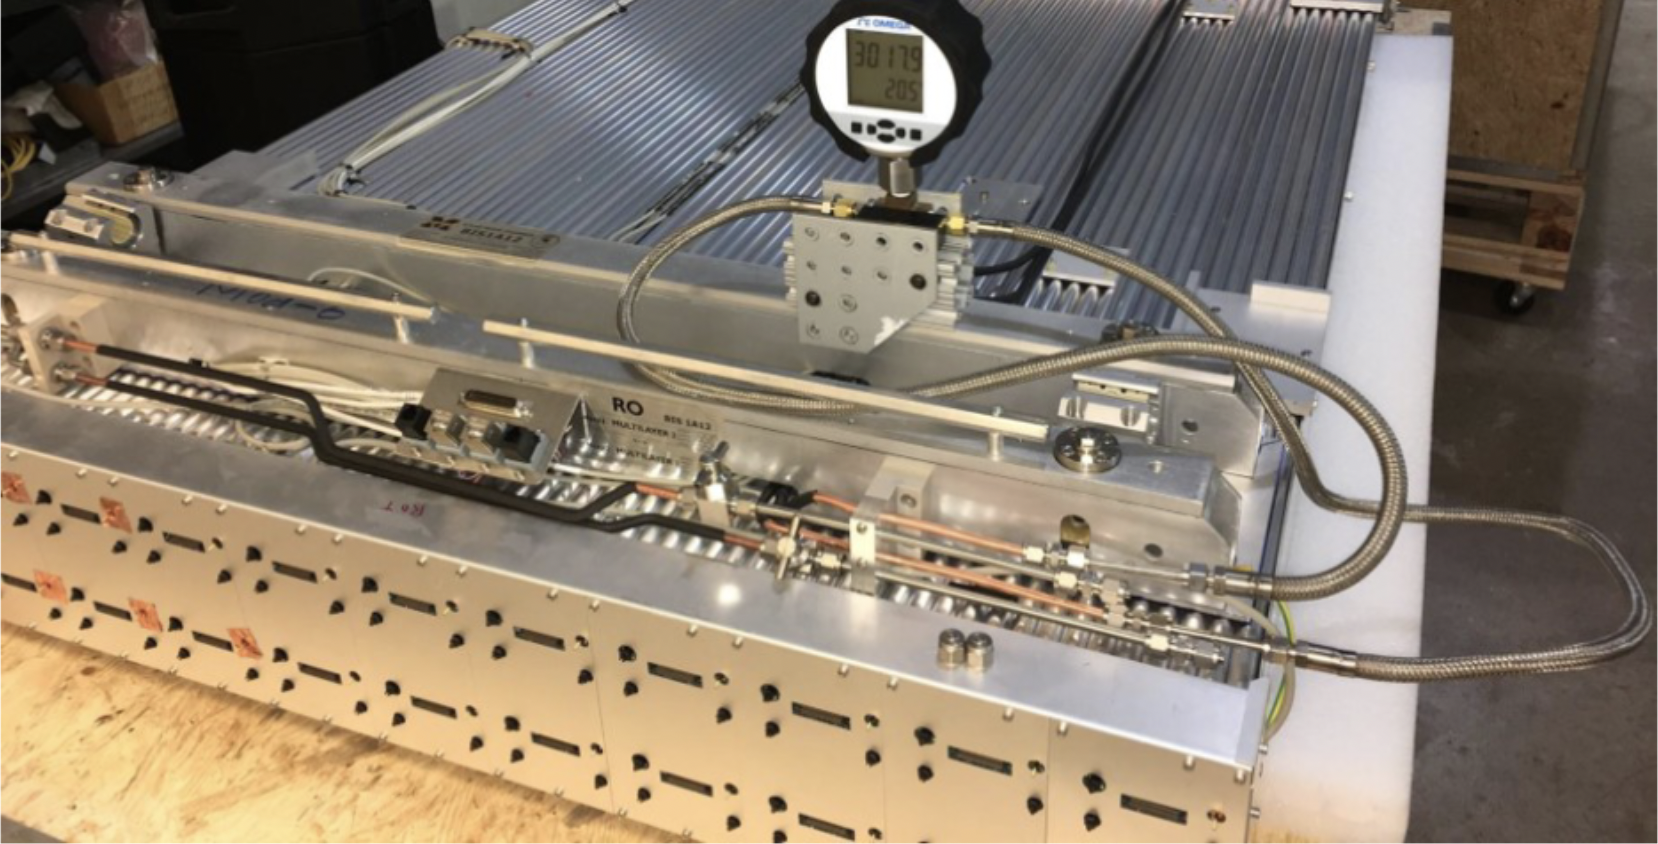
\includegraphics[width=0.5\pdfpagewidth]{PressureGauge.png}
		\end{figure}
		$$\Delta P_\text{corr}=P_f\frac{T_\text{ref}}{T_f}-P_i\frac{T_\text{ref}}{T_i}$$
	\end{frame}
	\begin{frame}{\hyperlinktarget{LeakRateTubes}{LeakRateTubesExtra}{Leak Rate Test - Tubes}}
		\begin{itemize}
			\item Ensures leak rate of individual tube is below 1E-5 mbar$\cdot$L/s.
			\item One tube at a time.
			\item Test takes $\sim2$ minutes.
			\item Tube is filled to 3 bar(a)
			\item Uses Leybold Quadro Phoenix Dry pump leak detector. 
		\end{itemize}
	\end{frame}
	\begin{frame}{\hyperlinktarget{TensionPhoto}{TensionExtra}{Tension - Extra}}
		\begin{itemize}
			\item Ensures tension of individual tube is between 325-380g.
			\item One tube at a time.
			\item Test takes $\sim30$ seconds.
			\item Tube is tested initially after construction, then tested 2 weeks after initial test. 
			\item Uses LabVIEW VI for signal generation and data collection.
		\end{itemize}
	\end{frame}
	\begin{frame}{\hyperlinktarget{DC}{DCExtra}{Dark Current - Extra}}
		\begin{itemize}
			\item Ensures noise rate of individual tube is below 2 nA.
			\item 48 tubes at a time.
			\item Test takes $\geq5$ hours.
			\item Tubes filled with 93:7 ArCO$_2$ at 3 bar(a), gas flowing at 1 SCFH. 
			\item Uses CAEN SY5527 power supply using CAEN GECO monitoring system.
		\end{itemize}
	\end{frame}
	\begin{frame}{Detailed UM Failure Rate}
		\begin{itemize}
			\item 19 Failed after construction during QA/QC tests. 
			\begin{itemize}
				\item 9 failed tension 
				\item 1 Leaked
				\item 1 had wire snap
				\item 1 had a crushed endpin.
				\item 1 had an electrical short
			\end{itemize}
			\item 44 raw tubes failed due to material deformities. (Bent, dent or deformities)
			\item 8 failed due to construction/mechanical errors that were seperate from normal testing.

		\end{itemize}
	\end{frame}
	\begin{frame}{DC Test - Extra}
		differences between tube test and chamber test
	\end{frame}
	\begin{frame}{Tension Test - Extra}
		Tension test is performed with LabVIEW.
	\end{frame}
\backupend
\end{document}

